% TeX root = ../main.tex

\section[Internet]{Internet}

\subsection{Arhitektura}

Predače Interneta kao što su ARPANET bile su u početku eksluzivne.
Broj korisnika bio je malen, ograničen na profesijonalne korisnike, uglavnom sveučilišta i vladine organizacije.
Stoga je i broj \textbf{čvorova} bio relativno mali.

Za razliku od ARPANET-a, na Internet su povezane milijarde uređaja, od osobnih računala, servera do pametnih automobila.
Očekuje da će broj ne-IoT uređaja povezanih na Internet (računala, serveri, itd.) u 2025.\ dostići 10 milijardi.
Sam broj uređaja je ogroman, veći je od populacije Zemlje, a svakom godinom se drastično povećava.

\definition{Čvor je fizičko računalo koje je član računalne mreže.}

\begin{figure}[h]\label{fig:arpanet}
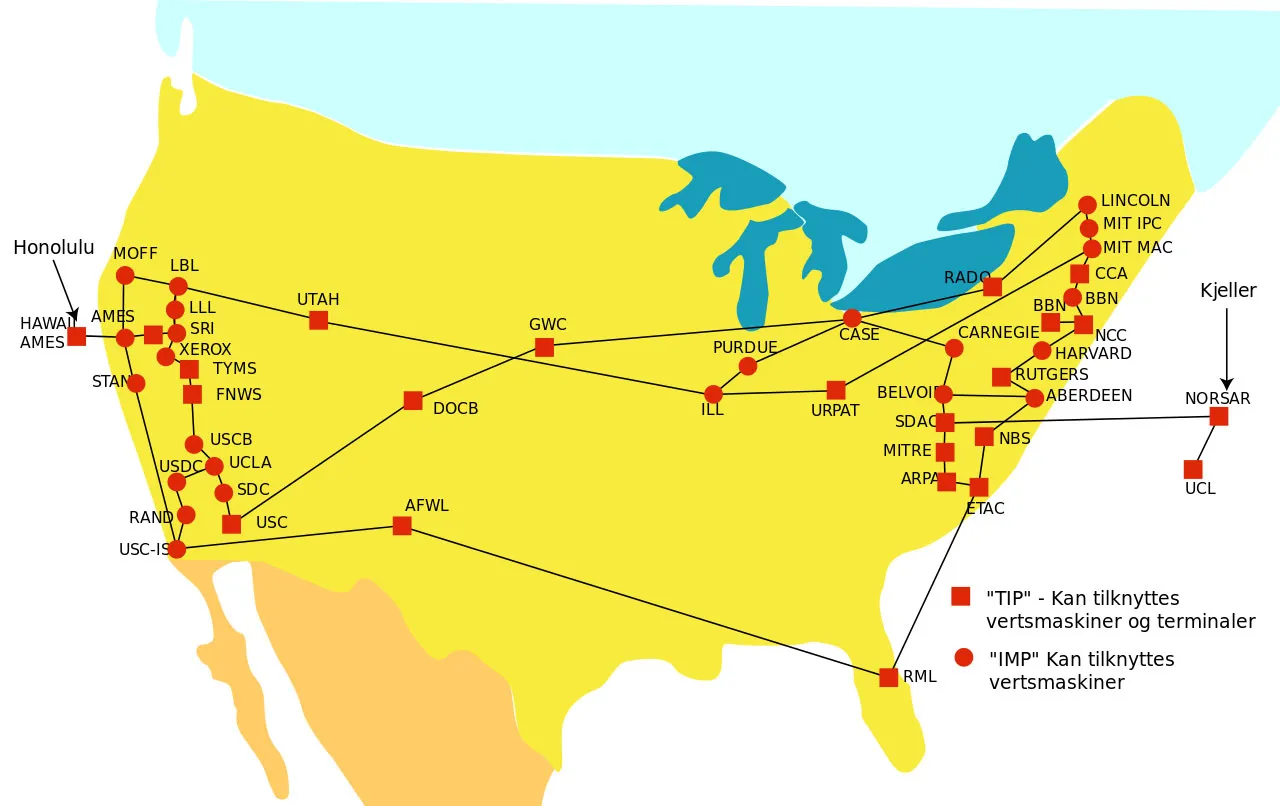
\includegraphics[scale=0.3125,left]{arpanet}
\raggedleft
\caption{Dijagram ARPANET mreže u rujnu 1974. Izvor: Britannica.}
\end{figure}

Dakle, zbog tolikog broja korisnika koje mora služiti, Internet mora biti dizajniran da podrži toliki broj korisnika.
Kao što smo prije spomenuli, Internet je masovni, distribuiran sustav.
Najlakše ga je zamisliti kao \textit{mrežu mreža}: ogromna mreža stvorena od velikog broja manjih mreža, npr. WAN, koje su same stvorene od još manjih mreža, npr. LAN.
Prostire se cijelom Zemljom, prolazi kroz stotine države i svih sedam kontinenata.

Internet načelno nema središnju organizaciju koja njime upravlja.
Malo je čudo što je moguće (na relativno lagan način) napraviti web stranicu kojoj netko može pristupiti putem Interneta iz (više-manje) bilo koje zemlje svijeta na gotovo bilo kojem uređaju s pristupom Internetu.
To je moguće zbog standardizacije koju provede međunarodne organizacije.

Jezgra Interneta sastoji se od nekoliko ogromnih, medunarodnih korporacija (ISP-ova) koji se vlasnici nekoliko skupina međusobno povezanih  mreža s velikim protokom.
Glavni dio tih mreža je skupina podvodnih komunikacijskih kablova koji povezuju Internet izmedu kontinenata.
Te mreže su \textbf{kralježnica Interneta}.
Ti su kablovi bitni geostrateški resursi za države, ali i korporacije.
Pomoću njih obavještajne agencije mogu provoditi kibernetičku špijunažu.\footnote{U SAD-u je ta agencija NSA, a u UK-u GCHQ.}

\begin{figure}[h]
    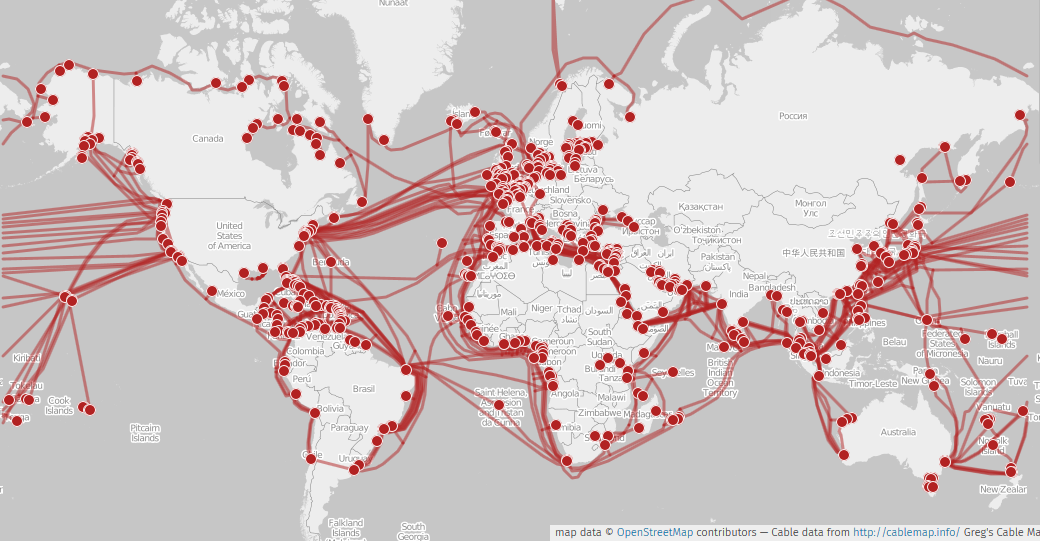
\includegraphics[scale = 0.42]{internet-underwater-backbone}
    \caption{Međukontinentalna mreža podvodnih komunikacijskih kablova koji služe kao kralježnica Interneta iz 2015. Izvor: OpenStreetMap. }\label{fig:figure6}
\end{figure}





\subsection{Adresiranje, domene i DNS}


\subsection{Mrežni protokoli}

\definition{Mrežni protokol je (obično standardizirani) skup pravila koja omogućuju koordinaciju i komunikaciju između dva ili više programa ili računala u mreži.}
